\documentclass[journal,12pt,twocolumn]{IEEEtran}
\usepackage{setspace}
\usepackage{gensymb}
\usepackage{caption}
%\usepackage{multirow}
%\usepackage{multicolumn}
%\usepackage{subcaption}
%\doublespacing
\singlespacing
\usepackage{csvsimple}
\usepackage{amsmath}
\usepackage{multicol}
%\usepackage{enumerate}
\usepackage{amssymb}
%\usepackage{graphicx}
\usepackage{newfloat}
%\usepackage{syntax}
\usepackage{listings}
\usepackage{iithtlc}
\usepackage{color}
\usepackage{tikz}
\usetikzlibrary{shapes,arrows}



%\usepackage{graphicx}
%\usepackage{amssymb}
%\usepackage{relsize}
%\usepackage[cmex10]{amsmath}
%\usepackage{mathtools}
%\usepackage{amsthm}
%\interdisplaylinepenalty=2500
%\savesymbol{iint}
%\usepackage{txfonts}
%\restoresymbol{TXF}{iint}
%\usepackage{wasysym}
\usepackage{amsthm}
\usepackage{mathrsfs}
\usepackage{txfonts}
\usepackage{stfloats}
\usepackage{cite}
\usepackage{cases}
\usepackage{mathtools}
\usepackage{caption}
\usepackage{enumerate}	
\usepackage{enumitem}
\usepackage{amsmath}
%\usepackage{xtab}
\usepackage{longtable}
\usepackage{multirow}
%\usepackage{algorithm}
%\usepackage{algpseudocode}
\usepackage{enumitem}
\usepackage{mathtools}
\usepackage{hyperref}
%\usepackage[framemethod=tikz]{mdframed}
\usepackage{listings}
    %\usepackage[latin1]{inputenc}                                 %%
    \usepackage{color}                                            %%
    \usepackage{array}                                            %%
    \usepackage{longtable}                                        %%
    \usepackage{calc}                                             %%
    \usepackage{multirow}                                         %%
    \usepackage{hhline}                                           %%
    \usepackage{ifthen}                                           %%
  %optionally (for landscape tables embedded in another document): %%
    \usepackage{lscape}     


\usepackage{url}
\def\UrlBreaks{\do\/\do-}


%\usepackage{stmaryrd}


%\usepackage{wasysym}
%\newcounter{MYtempeqncnt}
\DeclareMathOperator*{\Res}{Res}
%\renewcommand{\baselinestretch}{2}
\renewcommand\thesection{\arabic{section}}
\renewcommand\thesubsection{\thesection.\arabic{subsection}}
\renewcommand\thesubsubsection{\thesubsection.\arabic{subsubsection}}

\renewcommand\thesectiondis{\arabic{section}}
\renewcommand\thesubsectiondis{\thesectiondis.\arabic{subsection}}
\renewcommand\thesubsubsectiondis{\thesubsectiondis.\arabic{subsubsection}}

% correct bad hyphenation here
\hyphenation{op-tical net-works semi-conduc-tor}

%\lstset{
%language=C,
%frame=single, 
%breaklines=true
%}

%\lstset{
	%%basicstyle=\small\ttfamily\bfseries,
	%%numberstyle=\small\ttfamily,
	%language=Octave,
	%backgroundcolor=\color{white},
	%%frame=single,
	%%keywordstyle=\bfseries,
	%%breaklines=true,
	%%showstringspaces=false,
	%%xleftmargin=-10mm,
	%%aboveskip=-1mm,
	%%belowskip=0mm
%}

%\surroundwithmdframed[width=\columnwidth]{lstlisting}
\def\inputGnumericTable{}                                 %%
\lstset{
%language=C,
frame=single, 
breaklines=true,
columns=fullflexible
}
 

\begin{document}
%
\tikzstyle{block} = [rectangle, draw,
    text width=3em, text centered, minimum height=3em]
\tikzstyle{sum} = [draw, circle, node distance=3cm]
\tikzstyle{input} = [coordinate]
\tikzstyle{output} = [coordinate]
\tikzstyle{pinstyle} = [pin edge={to-,thin,black}]

\theoremstyle{definition}
\newtheorem{theorem}{Theorem}[section]
\newtheorem{problem}{Problem}
\newtheorem{proposition}{Proposition}[section]
\newtheorem{lemma}{Lemma}[section]
\newtheorem{corollary}[theorem]{Corollary}
\newtheorem{example}{Example}[section]
\newtheorem{definition}{Definition}[section]
%\newtheorem{algorithm}{Algorithm}[section]
%\newtheorem{cor}{Corollary}
\newcommand{\BEQA}{\begin{eqnarray}}
\newcommand{\EEQA}{\end{eqnarray}}
\newcommand{\define}{\stackrel{\triangle}{=}}

\bibliographystyle{IEEEtran}
%\bibliographystyle{ieeetr}

\providecommand{\nCr}[2]{\,^{#1}C_{#2}} % nCr
\providecommand{\nPr}[2]{\,^{#1}P_{#2}} % nPr
\providecommand{\mbf}{\mathbf}
\providecommand{\pr}[1]{\ensuremath{\Pr\left(#1\right)}}
\providecommand{\gauss}[2]{\mathcal{N}\ensuremath{\left(#1,#2\right)}}
\providecommand{\qfunc}[1]{\ensuremath{Q\left(#1\right)}}
\providecommand{\sbrak}[1]{\ensuremath{{}\left[#1\right]}}
\providecommand{\lsbrak}[1]{\ensuremath{{}\left[#1\right.}}
\providecommand{\rsbrak}[1]{\ensuremath{{}\left.#1\right]}}
\providecommand{\brak}[1]{\ensuremath{\left(#1\right)}}
\providecommand{\lbrak}[1]{\ensuremath{\left(#1\right.}}
\providecommand{\rbrak}[1]{\ensuremath{\left.#1\right)}}
\providecommand{\cbrak}[1]{\ensuremath{\left\{#1\right\}}}
\providecommand{\lcbrak}[1]{\ensuremath{\left\{#1\right.}}
\providecommand{\rcbrak}[1]{\ensuremath{\left.#1\right\}}}
\theoremstyle{remark}
\newtheorem{rem}{Remark}
\newcommand{\sgn}{\mathop{\mathrm{sgn}}}
\providecommand{\abs}[1]{\left\vert#1\right\vert}
\providecommand{\res}[1]{\Res\displaylimits_{#1}} 
\providecommand{\norm}[1]{\left\Vert#1\right\Vert}
\providecommand{\mtx}[1]{\mathbf{#1}}
\providecommand{\mean}[1]{E\left[ #1 \right]}
\providecommand{\fourier}{\overset{\mathcal{F}}{ \rightleftharpoons}}
%\providecommand{\hilbert}{\overset{\mathcal{H}}{ \rightleftharpoons}}
\providecommand{\system}{\overset{\mathcal{H}}{ \longleftrightarrow}}
	%\newcommand{\solution}[2]{\textbf{Solution:}{#1}}
\newcommand{\solution}{\noindent \textbf{Solution: }}
\newcommand{\myvec}[1]{\ensuremath{\begin{pmatrix}#1\end{pmatrix}}}
\providecommand{\dec}[2]{\ensuremath{\overset{#1}{\underset{#2}{\gtrless}}}}
\DeclarePairedDelimiter{\ceil}{\lceil}{\rceil}
%\numberwithin{equation}{section}
%\numberwithin{problem}{subsection}
%\numberwithin{definition}{subsection}
\makeatletter
\@addtoreset{figure}{section}
\makeatother

\let\StandardTheFigure\thefigure
%\renewcommand{\thefigure}{\theproblem.\arabic{figure}}
\renewcommand{\thefigure}{\thesection}


%\numberwithin{figure}{subsection}

%\numberwithin{equation}{subsection}
%\numberwithin{equation}{section}
%\numberwithin{equation}{problem}
%\numberwithin{problem}{subsection}
\numberwithin{problem}{section}
%%\numberwithin{definition}{subsection}
%\makeatletter
%\@addtoreset{figure}{problem}
%\makeatother
\makeatletter
\@addtoreset{table}{section}
\makeatother

\let\StandardTheFigure\thefigure
\let\StandardTheTable\thetable
\let\vec\mathbf
\numberwithin{equation}{section}

\vspace{3cm}


\title{%Convex Optimization in Python
	\logo{
	Random Numbers
	}
}
%\title{
%	\logo{Matrix Analysis through Octave}{\begin{center}\includegraphics[scale=.24]{tlc}\end{center}}{}{HAMDSP}
%}


% paper title
% can use linebreaks \\ within to get better formatting as desired
%\title{Matrix Analysis through Octave}
%
%
% author names and IEEE memberships
% note positions of commas and nonbreaking spaces ( ~ ) LaTeX will not break
% a structure at a ~ so this keeps an author's name from being broken across
% two lines.
% use \thanks{} to gain access to the first footnote area
% a separate \thanks must be used for each paragraph as LaTeX2e's \thanks
% was not built to handle multiple paragraphs
%

\author{ Rahul Ramachandran
%  $^{*}$% <-this % stops a space
% \thanks{* The author is with the Department
% of Electrical Engineering, Indian Institute of Technology, Hyderabad
% 502285 India e-mail:  gadepall@iith.ac.in.}% <-this % stops a space
%\thanks{J. Doe and J. Doe are with Anonymous University.}% <-this % stops a space
%\thanks{Manuscript received April 19, 2005; revised January 11, 2007.}}
}
% note the % following the last \IEEEmembership and also \thanks - 
% these prevent an unwanted space from occurring between the last author name
% and the end of the author line. i.e., if you had this:
% 
% \author{....lastname \thanks{...} \thanks{...} }
%                     ^------------^------------^----Do not want these spaces!
%
% a space would be appended to the last name and could cause every name on that
% line to be shifted left slightly. This is one of those "LaTeX things". For
% instance, "\textbf{A} \textbf{B}" will typeset as "A B" not "AB". To get
% "AB" then you have to do: "\textbf{A}\textbf{B}"
% \thanks is no different in this regard, so shield the last } of each \thanks
% that ends a line with a % and do not let a space in before the next \thanks.
% Spaces after \IEEEmembership other than the last one are OK (and needed) as
% you are supposed to have spaces between the names. For what it is worth,
% this is a minor point as most people would not even notice if the said evil
% space somehow managed to creep in.



% The paper headers
%\markboth{Journal of \LaTeX\ Class Files,~Vol.~6, No.~1, January~2007}%
%{Shell \MakeLowercase{\textit{et al.}}: Bare Demo of IEEEtran.cls for Journals}
% The only time the second header will appear is for the odd numbered pages
% after the title page when using the twoside option.
% 
% *** Note that you probably will NOT want to include the author's ***
% *** name in the headers of peer review papers.                   ***
% You can use \ifCLASSOPTIONpeerreview for conditional compilation here if
% you desire.




% If you want to put a publisher's ID mark on the page you can do it like
% this:
%\IEEEpubid{0000--0000/00\$00.00~\copyright~2007 IEEE}
% Remember, if you use this you must call \IEEEpubidadjcol in the second
% column for its text to clear the IEEEpubid mark.



% make the title area
\maketitle

\tableofcontents

\bigskip

\renewcommand{\thefigure}{\theenumi}
\renewcommand{\thetable}{\theenumi}

\begin{abstract}
This manual provides a simple introduction to the generation of random numbers
\end{abstract}
%%
\section{Uniform Random Numbers}
Let $U$ be a uniform random variable between 0 and 1.
\begin{enumerate}[label=\thesection.\arabic*
,ref=\thesection.\theenumi]
\item Generate $10^6$ samples of $U$ using a C program and save into a file called uni.dat .
\\
\solution Download the following files and execute the  C program.
\begin{lstlisting}
wget https://github.com/gadepall/probability/raw/master/manual/codes/exrand.c
wget https://github.com/gadepall/probability/raw/master/manual/codes/coeffs.h
gcc exrand.c
./a.out
\end{lstlisting}

%
\item
Load the uni.dat file into python and plot the empirical CDF of $U$ using the samples in uni.dat. The CDF is defined as
\begin{align}
F_{U}(x) = \pr{U \le x}
\end{align}
\\
\solution \begin{lstlisting}
wget https://github.com/gadepall/probability/raw/master/manual/codes/cdf_plot.py
python3 cdf_plot.py
\end{lstlisting}
\begin{figure}
\centering
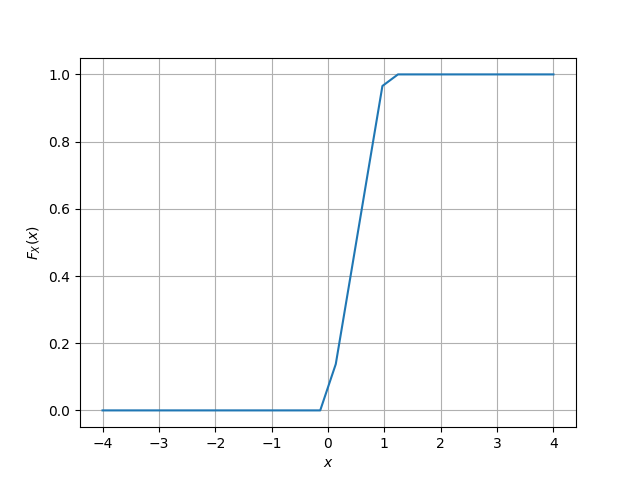
\includegraphics[width=\columnwidth]{./figures/CDF_uni.png}
\caption{The CDF of $U$}
\label{fig:uni_cdf}
\end{figure}
 The following code plots Fig. \ref{fig:uni_cdf}

%
\item
Find a  theoretical expression for $F_{U}(x)$.
\\
\solution
$U$ is given by 
\begin{align}
    U(x) = 
    \begin{cases}
        0, & x \in (-\infty,0) \\
        1, & x \in (0,1) \\
        0, & x \in (1, \infty)
    \end{cases}
\end{align}
Therefore, we have:
    \begin{align}
        F_U(x) = \int_0^x U(x) dx
    \end{align}
Computing the integral, we get:

\begin{align}
    F_U(x) = 
    \begin{cases}
        0, & x \in (-\infty,0) \\
        x, & x \in (0,1) \\
        1, & x \in (1, \infty)
    \end{cases}
\end{align}


\item
The mean of $U$ is defined as
%
\begin{equation}
E\sbrak{U} = \frac{1}{N}\sum_{i=1}^{N}U_i
\end{equation}
%
and its variance as
%
\begin{equation}
\text{var}\sbrak{U} = E\sbrak{U- E\sbrak{U}}^2 
\end{equation}

Write a C program to  find the mean and variance of $U$. 

\\
\solution
Add the following function to coeffs.h
\begin{lstlisting}
    double variance(char *str)
{
int i=0,c;
FILE *fp;
double x, temp=0.0;

fp = fopen(str,"r");
//get numbers from file
while(fscanf(fp,"%lf",&x)!=EOF)
{
//Count numbers in file
i=i+1;
//Add all numbers in file
temp = temp+x*x;
}
double mn = mean(str);
fclose(fp);
temp = temp/(i-1);
return temp - mn*mn ;

}
    \end{lstlisting}

Following the steps mentioned below gives the required result:

\begin{lstlisting}
    gcc exrand.c
    ./a.out
    mean = 0.500031
    variance = 0.083247
\end{lstlisting}






\item Verify your result theoretically given that
\end{enumerate}
%
\begin{equation}
E\sbrak{U^k} = \int_{-\infty}^{\infty}x^kdF_{U}(x)
\end{equation}
\\
\solution  Since 
\begin{align}
    dF_U(x) = p_U(x) dx
\end{align}
we have:
\begin{align}
    \label{eq2}
    E[U^k] = \int_{-\infty}^{\infty}x^k p_U(x) dx
\end{align}
Also,
\begin{align}
    \label{eq3}
     p_U(x) = 
    \begin{cases}
        0, & x \in (-\infty,0) \\
        1, & x \in (0,1) \\
        0, & x \in (1, \infty)
    \end{cases}
\end{align}

Therefore, from Equations \ref{eq2} and \ref{eq3}, we have:
    
    \begin{align}
        E[U^2] &=  \int_{-\infty}^{\infty}x^2 p_U(x) dx \\
        &= \int_0 ^1 x^2 dx \\
        &= \frac{1}{3}
    \end{align}
    
    Similarly, 
    \begin{align}
        E[U] &=  \int_{-\infty}^{\infty}x p_U(x) dx \\
        &= \int_0 ^1 x dx \\
        &= \frac{1}{2}
    \end{align}

    Therefore, the mean is $\frac{1}{2}$, and the variance equals:
    \begin{align}
        E[U^2] - E[U]^2 &= \frac{1}{3} - \brak{\frac{1}{2}}^2 \\
        &= \frac{1}{12}
    \end{align}


\section{Central Limit Theorem}
%
\begin{enumerate}[label=\thesection.\arabic*
,ref=\thesection.\theenumi]

%
\item
Generate $10^6$ samples of the random variable
%
\begin{equation}
X = \sum_{i=1}^{12}U_i -6
\end{equation}
%
using a C program, where $U_i, i = 1,2,\dots, 12$ are  a set of independent uniform random variables between 0 and 1
and save in a file called gau.dat
\\
\solution
Add the following line to \textbf{exrand.c} and execute the code:
\begin{lstlisting}
    gaussian("gau.dat", 1000000);
    gcc exrand.c
    ./a.out
\end{lstlisting}

%
\item
Load gau.dat in python and plot the empirical CDF of $X$ using the samples in gau.dat. What properties does a CDF have?
\\
\solution 




The CDF of $X$ is plotted in Fig. \ref{fig:gauss_cdf}
\begin{figure}
\centering
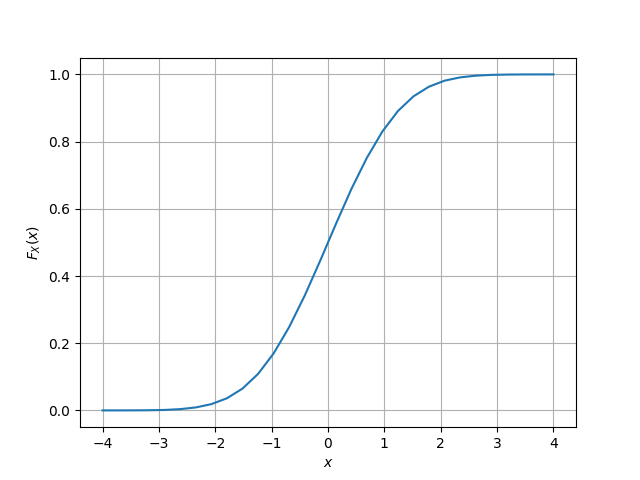
\includegraphics[width=\columnwidth]{./figures/CDF_gau.png}
\caption{The CDF of $X$}
\label{fig:gauss_cdf}
\end{figure}


\item
Load gau.dat in python and plot the empirical PDF of $X$ using the samples in gau.dat. The PDF of $X$ is defined as
\begin{align}
p_{X}(x) = \frac{d}{dx}F_{X}(x)
\end{align}
What properties does the PDF have?
\\
\solution The PDF of $X$ is plotted in Fig. \ref{fig:gauss_pdf} using the code below
\begin{lstlisting}
wget https://github.com/gadepall/probability/raw/master/manual/codes/pdf_plot.py
python3 pdf_plot.py
\end{lstlisting}

\begin{figure}
\centering
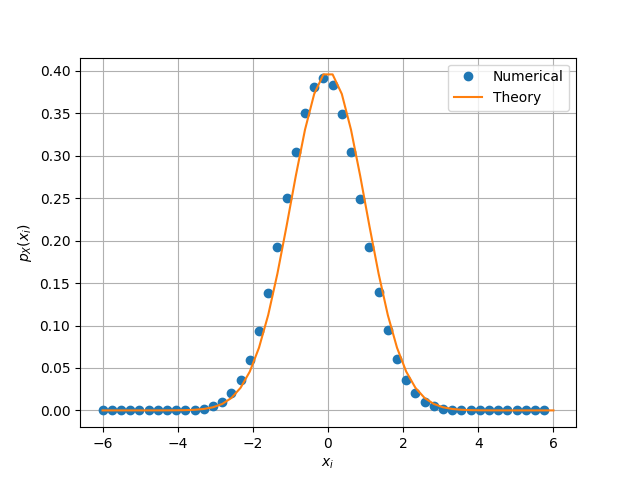
\includegraphics[width=\columnwidth]{./figures/PDF_gau.png}
\caption{The PDF of $X$}
\label{fig:gauss_pdf}
\end{figure}

To find the CDF theoretically, consider




\item Find the mean and variance of $X$ by writing a C program.
\\
\solution Use the main and variance functions in \textbf{coeffs.h}, and execute the code below
\begin{lstlisting}
    gcc exrand.c
    ./a.out
\end{lstlisting}
We get
\begin{lstlisting}
    mean = 0.000685
    variance = 1.000025
\end{lstlisting}


\item Given that 
\begin{align}
p_{X}(x) = \frac{1}{\sqrt{2\pi}}\exp\brak{-\frac{x^2}{2}}, -\infty < x < \infty,
\end{align}
repeat the above exercise theoretically.
\\
\solution  We have:
    
\begin{align}
    E[X] &=  \int_{-\infty}^{\infty} \frac{x}{\sqrt{2\pi}}\exp{\left(-\frac{x^2}{2}\right)} \\
    &= -\frac{1}{\sqrt{2\pi}}\exp\brak{-\frac{x^2}{2}} \Bigg{|}_{-\infty}^{\infty} \\
    &= 0 
\end{align}

Also,
    
\begin{align}
    E[X^2] &=  \int_{-\infty}^{\infty} \frac{x^2}{\sqrt{2\pi}}\exp{\left(-\frac{x^2}{2}\right)} \\
    &= -\frac{x}{\sqrt{2\pi}}e^{\brak{-\frac{x^2}{2}}} \Bigg{|}_{-\infty}^{\infty} + \int_{-\infty}^{\infty} \frac{1}{\sqrt{2\pi}}e^{\brak{-\frac{x^2}{2}}}   \\
    &= 0 + \frac{1}{\sqrt{2\pi}} \times \sqrt{2\pi} \\
    &= 1
\end{align}

Hence, 

\begin{align}
    \text{var}(X) &= E[X^2] - E[X]^2 \\ 
    &= 1 
\end{align}

Therefore, the mean is $0$ and the variance is $1$. Running the empirical code in \textbf{./codes/exrancd.c}, 
   we get mean = $0.000685$ and variance = $1.000025$, which closely matches the theoretical values.


\item Find the theoretical CDF of $X$
\\
\solution
 To find the theoretical CDF, consider:

\begin{align}
    Q_X(x) &= \int_x ^{\infty} \frac{1}{\sqrt{2\pi}} e^{\frac{-x^2}{2}} dx \\
      &= \frac{\text{erfc}(\frac{x}{\sqrt{2}})}{2}
   \end{align}

The CDF is then:
\begin{align}
    F_X(x) &= 1 - Q_X(x) \\
    &= 1 - \frac{\text{erfc}(\frac{x}{\sqrt{2}})}{2}
\end{align}

%
\end{enumerate}
\section{From Uniform to Other}
\begin{enumerate}[label=\thesection.\arabic*
,ref=\thesection.\theenumi]
%
\item
Generate samples of 
%
\begin{equation}
V = -2\ln\brak{1-U}
\end{equation}
%
and plot its CDF.  
\solution 

Add the following function to \textbf{coeffs.h}:
\begin{lstlisting}
    void logarithmic(char *str){
  int i=0,c;
FILE *fp, *fp2;
double x, temp=0.0;

fp = fopen("uni.dat","r");
fp2 = fopen(str, "w");
//get numbers from file
while(fscanf(fp,"%lf",&x)!=EOF)
{
  temp = -2*log(1-x);
  fprintf(fp2,"%lf\n",temp);
}

fclose(fp);
fclose(fp2);

return ;

}
    \end{lstlisting}

Using this function in \textbf{exrand.c} prints the numbers in 
\textbf{log.dat} 


\item Find a theoretical expression for $F_V(x)$.
\\
\solution  We have:
    
\begin{align}
F_V(x) &= \pr{V \leq x} \\
&= \pr{-2\ln(1-U) \leq x} \\
&= \pr{1-U \geq	\exp{\left(-\frac{x}{2}\right)}} \\
&= \pr{U \leq 1 - \exp{\left(-\frac{x}{2}\right)}} \\
&= F_U\left(1 - \exp{\left(-\frac{x}{2}\right)}\right) 
\end{align}

Therefore,
    \begin{align}
       F_V(x) =
        \begin{cases}
            0, & 1 - \exp{\left(-\frac{x}{2}\right)} \in (-\infty,0) \\
            1 - \exp{\left(-\frac{x}{2}\right)}, & 1 - \exp{\left(-\frac{x}{2}\right)} \in (0,1) \\
            1, & 1 - \exp{\left(-\frac{x}{2}\right)} \in (1, \infty)
        \end{cases}
    \end{align}
    
    From this we get:
    
    \begin{align}
       F_V(x) =
        \begin{cases}
            0, & x \in (-\infty,0) \\
            1 - \exp{\left(-\frac{x}{2}\right)}, & x \in (0,\infty) 
        \end{cases}
    \end{align}

    \begin{figure}
        \centering
        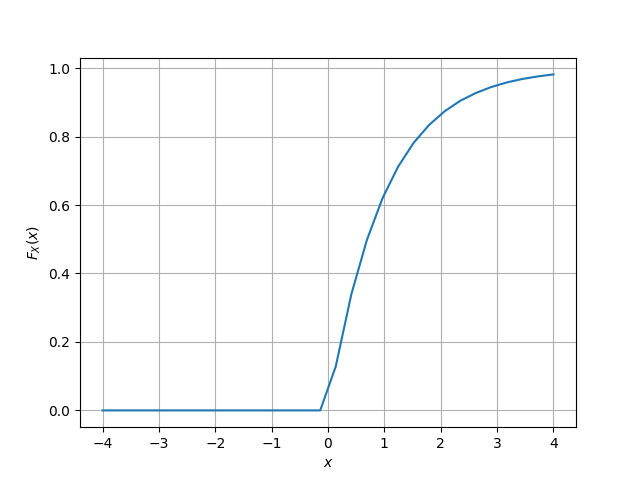
\includegraphics[width=\columnwidth]{./figures/CDF_log.png}
        \caption{The CDF of $V$}
        \label{fig:log_cdf}
        \end{figure}
    The CDF of $V$ is plotted in Fig. \ref{fig:log_cdf}

%
%\item
%Generate the Rayleigh distribution from Uniform. Verify your result through graphical plots.

    \end{enumerate}




\section{Triangular Distributions}
\begin{enumerate}[label=\thesection.\arabic*
    ,ref=\thesection.\theenumi]
\item Generate 
	\begin{align}
		T = U_1+U_2
	\end{align}
\\
\solution Use the function 'triangular' in \textbf{exrand.c} and execute the following code:
\begin{lstlisting}
wget https://github.com/Rahuboy/AI1110/blob/main/RandomNumbers/codes/coeffs.h
wget https://github.com/Rahuboy/AI1110/blob/main/RandomNumbers/codes/exrand.c
gcc exrand.c
./a.out
    \end{lstlisting}

\item Find the CDF of $T$.
\\

\solution  

\begin{lstlisting}
    wget https://github.com/Rahuboy/AI1110/blob/main/RandomNumbers/codes/cdf_plot.py
    python3 cdf_plot.py
    \end{lstlisting}
  
    \begin{figure}
        \centering
        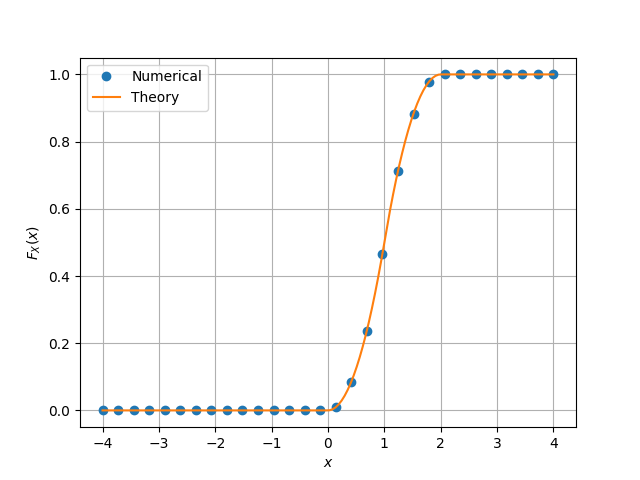
\includegraphics[width=\columnwidth]{./figures/CDF_tri.png}
        \caption{The CDF of $T$}
        \label{fig:tri_cdf}
        \end{figure}

        The above code plots Fig. \ref{fig:tri_cdf}

\item Find the PDF of $T$.

\begin{lstlisting}
    wget https://github.com/Rahuboy/AI1110/blob/main/RandomNumbers/codes/pdf_plot.py
    python3 pdf_plot.py
    \end{lstlisting}

  
    \begin{figure}
        \centering
        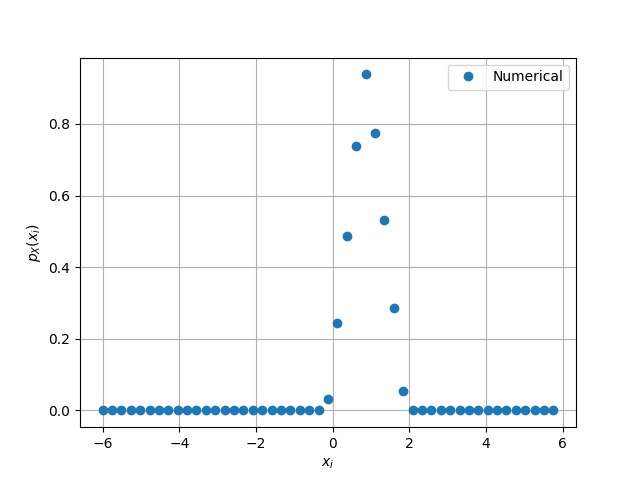
\includegraphics[width=\columnwidth]{./figures/PDF_tri.png}
        \caption{The PDF of $T$}
        \label{fig:tri_pdf}
        \end{figure}

        The above code plots Fig. \ref{fig:tri_pdf}
 
\item Find the theoretical expressions for the PDF and CDF of $T$.
\\
\solution When 
\begin{align}
    Z = X + Y
\end{align}
where X, Y and Z are random variables, we have:
\begin{align}
    p_Z(t) &= (p_X * p_Y)(t) \\
    &= \int _{-\infty} ^{\infty} p_X(\tau) p_Y(t-\tau) d\tau
\end{align}

Here, $p_X(t) = p_Y(t) = p_U(t) $. Therefore:
\begin{align}
    p_T(t) &= \int _{-\infty} ^{\infty} p_U(\tau) p_U(t-\tau) d\tau \\
    &= \int _0 ^1 p_U(t-\tau) d\tau
\end{align}

When $t < 0$ and $t > 2$ , the integral evaluates to $0$. When $0 < t < 1$:
\begin{align}
    p_T(t)  &= \int _0 ^1 p_U(t-\tau) d\tau \\
    &= \int _0 ^t p_U(t-\tau) d\tau \\
    &= \int _0 ^t 1 d\tau \\
    &= t
\end{align}

when $ 1 < t < 2$:
\begin{align}
    p_T(t)  &= \int _0 ^1 p_U(t-\tau) d\tau \\
    &= \int _{t-1} ^1 p_U(t-\tau) d\tau \\
    &= \int _{t-1} ^1 1 d\tau \\
    &= 2-t
\end{align}

Therefore, we have:
\begin{align}
    p_T(x) = 
    \begin{cases}
        0, & x \in (-\infty,0) \\
        x, & x \in (0,1) \\
        2-x, & x \in (1, 2) \\
        0, & x \in (2,\infty)
    \end{cases}
\end{align}

To find the CDF, we use:
\begin{align}
    F_T(x) = \int _{-\infty} ^x p_T(t) dt
\end{align}

We get:
\begin{align}
    F_T(x) = 
    \begin{cases}
        0, & x \in (-\infty,0) \\
        \frac{x^2}{2}, & x \in (0,1) \\
        -\frac{x^2}{2} + 2x - 1, & x \in (1, 2) \\
        1, & x \in (2,\infty)
    \end{cases}
\end{align}


\item Verify your result for the PDF through a plot. 
\\
\solution Execute the following code:
\begin{lstlisting}
    python3 pdf_plot.py
\end{lstlisting}

\begin{figure}
    \centering
    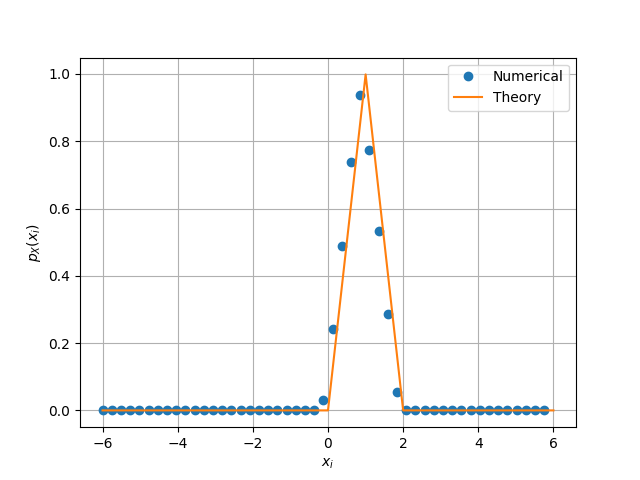
\includegraphics[width=\columnwidth]{./figures/PDF_tri_sim.png}
    \caption{The PDF of $T$}
    \label{fig:tri_pdf_sim}
    \end{figure}

    The theoretical PDF is plotted in Fig. \ref{fig:tri_pdf_sim}    

    \item Verify your result for the CDF through a plot. 
\\
\solution Execute the following code:
\begin{lstlisting}
    python3 cdf_plot.py
\end{lstlisting}

The theoretical CDF is plotted in Fig. \ref{fig:tri_cdf_sim}    
    

\begin{figure}
    \centering
    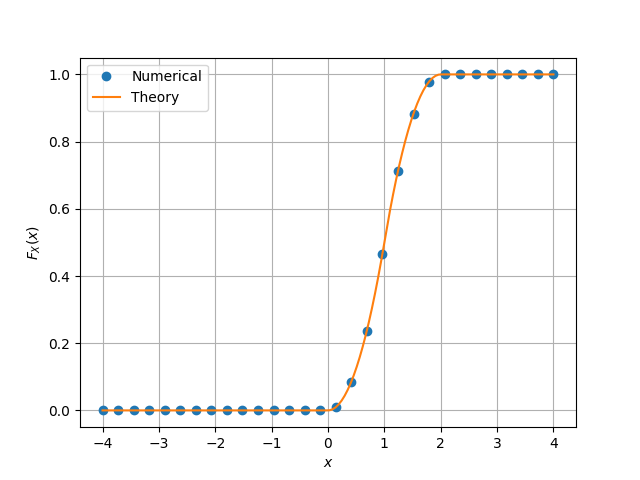
\includegraphics[width=\columnwidth]{./figures/CDF_tri_sim.png}
    \caption{The CDF of $T$}
    \label{fig:tri_cdf_sim}
    \end{figure}

   
\end{enumerate}







\section{Maximal Likelihood}
\begin{enumerate}[label=\thesection.\arabic*
    ,ref=\thesection.\theenumi]


    \item Generate equiprobable $X \in \cbrak{1,-1}$.
    \\
    \solution
    Use the function "bernoulli" in \textbf{exrand.c} and execute the code below:
    \begin{lstlisting}
        gcc exrand.c
        ./a.out
    \end{lstlisting}



\item Generate 
    \begin{equation}
    Y = AX+N,
    \end{equation}
            where $A = 5 \text{ dB}, X \i \cbrak{1,-1}$,  is Bernoulli and $N \sim \gauss{0}{1}$.
    \\
    \solution Use the functions 'bernoulli' and 'maxlike' in \textbf{exrand.c}:

\begin{lstlisting}
    gcc exrand.c
    ./a.out
\end{lstlisting}



\item Plot $Y$.

\begin{figure}
    \centering
    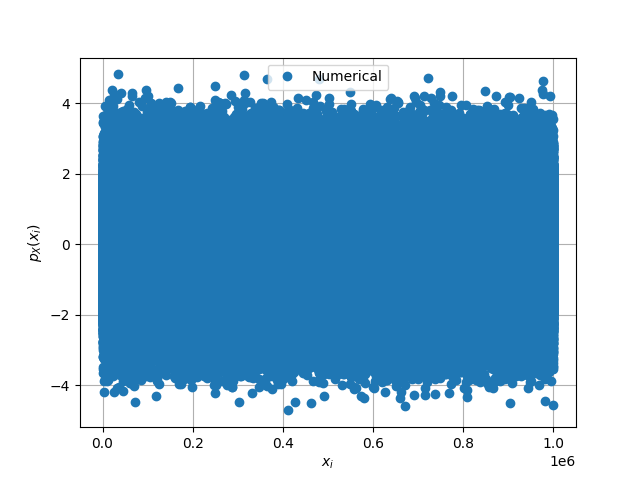
\includegraphics[width=\columnwidth]{./figures/Noise.png}
    \caption{The Plot of $Y$}
    \label{fig:noise}
    \end{figure}

    Y is plotted in Fig. \ref{fig:noise}  




    \item Guess how to estimate $X$ from $Y$.
\\
\solution To estimate $X$ from $Y$, we define the following function:

\begin{align}
    \sgn(y) = 
    \begin{cases}
        -1, & y \in (-\infty,0] \\
        1, & y \in (0, \infty)
    \end{cases}
\end{align}

Using $\sgn{y}$, we can operate on $Y$ to find corresponding values of $X$.




\item
\label{ml-ch4_sim}
Find 
\begin{equation}
	P_{e|0} = \pr{\hat{X} = -1|X=1}
\end{equation}
and 
\begin{equation}
	P_{e|1} = \pr{\hat{X} = 1|X=-1}
\end{equation}

\\
\solution Use the function "maxlike\_proberr" in \textbf{exrand.c} to find the respective probabilities:

\begin{lstlisting}
gcc exrand.c
./a.out
P_(e|0) = 0.312414
P_(e|1) = 0.310985
\end{lstlisting}




\item Find $P_e$.
\\
\solution
Assume a general value of $A$. Our estimation function predicts that the data points above the $x$ axis
correspond to $X=1$, and the data points below the $x$-axis correspond to $X=-1$. This isn't always the case,
as $Y=AX+N$, and the $N$ causes some spill-over.
We have:
\begin{align}
    P_{e|0} &= \pr{\hat{X} = -1|X=1} \\
    &= \pr{AX+N<0|X=1} \\
    &= \pr{N<-A} \\
    &= \int_{-\infty} ^{-A} \frac{1}{\sqrt{2\pi}} e^{\frac{-x^2}{2}} dx \\
    &= \int_{A} ^{\infty} \frac{1}{\sqrt{2\pi}} e^{\frac{-x^2}{2}} dx \\
    &= Q_N(A)
\end{align}
where $Q\_N$ is the $Q-$function of the normal distribution.

Similarly, 
\begin{align}
    P_{e|1} = Q_N(A)
\end{align}

Therefore, 
\begin{align}
    P_e &= P_{e|0} \times \pr{X=1} + P_{e|1} \times \pr{X=-1} \\
    &= \frac{1}{2} P_{e|0} + \frac{1}{2} P_{e|1} \\
    &= \frac{1}{2} Q_N(A) + \frac{1}{2} Q_N(A) \\
    &= Q_N(A)
\end{align}


\item
Verify by plotting  the theoretical $P_e$.  
\\
\solution
The graph of $P_e$ is plotted in Fig. \ref{fig:errorgraph}  

\begin{figure}
    \centering
    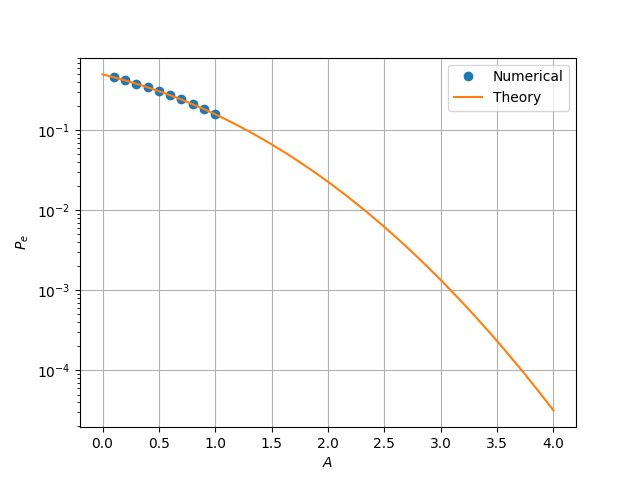
\includegraphics[width=\columnwidth]{./figures/ErrorGraph.png}
    \caption{The Plot of $P_e$}
    \label{fig:errorgraph}
    \end{figure}



\item Now, consider a threshold $\delta$  while estimating $X$ from $Y$. Find the value of $\delta$ that maximizes the theoretical $P_e$.
\\
\solution
To estimate $X$ from $Y$, we now consider the following:
\begin{align}
    X = 
    \begin{cases}
        1, & Y > \delta \\
        -1, & Y < \delta
    \end{cases}
\end{align}
Therefore,

\begin{align}
P_{e|0} &= \pr{\hat{X} = -1 | X = 1} \\
&= \pr{AX+N < \delta | X = 1} \\
&= \pr{N < \delta - A} \\
&= \int _{-\infty} ^{\delta - A} \frac{1}{\sqrt{2\pi}} e^{-\frac{x^2}{2}} dx \\
&= \int _{A - \delta} ^{\infty} \frac{1}{\sqrt{2\pi}} e^{-\frac{x^2}{2}} dx \\
&= Q_N(A - \delta) \\
\intertext{Where $Q\_N$ is the $Q$-function of the normal distribution. Similarly,}
P_{e|1} &= Q_N(A+\delta) \\
\intertext{Therefore,}
\label{eq:Pe_equation}
P_e &= P_{e|0} \pr{X = 1} + P_{e|1} \pr{X = -1} \\
&= \frac{1}{2}(Q_N(A - \delta) + Q_N(A + \delta)) \\
\end{align}

To minimise $P\_e$, we differentiate the above equation wrt $\delta$:

\begin{align}
0 &= \frac{d}{d\delta} \left(\frac{1}{2}(Q_N(A - \delta) + Q_N(A + \delta))\right) \\
&= \frac{1}{2} (\frac{1}{\sqrt{2\pi}} e^{-\frac{(\delta - A)^2}{2}} - \frac{1}{\sqrt{2\pi}} e^{-\frac{(A + \delta)^2}{2}} ) \\
\intertext{Therefore,}
(\delta - A)^2 &= (\delta + A)^2 \\
\implies \delta &= 0
\end{align}






\item Repeat the above exercise when 
    \begin{align}
        p_{X}(0) = p
    \end{align}
\\
\solution
Using Eq. \eqref{eq:Pe_equation}, we have:

\begin{align}
    P_e &= P_{e|0} p+ P_{e|1} (1-p) \\
    &= p Q_N(A - \delta) + (1-p)Q_N(A + \delta)
\intertext{Differentiating as before, we get:}
0 &= p \frac{1}{\sqrt{2\pi}} e^{-\frac{(\delta - A)^2}{2}} - (1-p)\frac{1}{\sqrt{2\pi}} e^{-\frac{(A + \delta)^2}{2}} 
\end{align}
 Taking $\ln$ on both sides we have:

 \begin{align}
    \ln{p} - \frac{(\delta - A)^2}{2} &= \ln{1-p} + \frac{(\delta + A)^2}{2} \\
    \implies \delta &= \frac{1}{2A} \ln{\frac{1-p}{p}}
 \end{align}



    \item Repeat the above exercise using the MAP criterion.
\\
\solution
Assume that $\pr{X = -1} = p$, and $\pr{X = 1} = (1-p)$. Then, using the Law of Total Probability,
we have:

\begin{align}
\nonumber p_Y(y) &= p_{Y|X = -1}(y|-1) \pr{X = -1} \\
&+ p_{Y| X = 1}(y|1) \pr{X = 1} \\
\nonumber &= p \times p_{(-A + N)}(y) \\
&+ (1-p) \times p_{(A+N)} (y) 
\end{align}
 
where $p_Y(y)$ is the pdf of $Y$. Now, $p_{(-A + N)}$ is just the pdf of a shifted
normal distribution, and therefore:

\begin{align}
    p_Y(y) &=  p \frac{e^{-\frac{(y+A)^2}{2}}}{\sqrt{2\pi}} + \left(1-p\right) \frac{e^{-\frac{(y-A)^2}{2}}}{\sqrt{2\pi}}
\end{align}

To use the MAP criterion, we must find $p_{X|Y}(x|y)$. To do this, we use the Theorem of Conditional Probability:

\begin{align}
    p_{X|Y}(x|y) &= \frac{p_{Y|X}(y|x) \times p_X(x)}{p_Y(y)}
\end{align}

When $X=1$, we have:

\begin{align}
    p_{X|Y}(1|y) &= \frac{p_{Y|X}(y|1) \times p_X(1)}{p_Y(y)} \\
    &= \frac{\left(1-p\right) \frac{e^{-\frac{(y-A)^2}{2}}}{\sqrt{2\pi}}}{ p \frac{e^{-\frac{(y+A)^2}{2}}}{\sqrt{2\pi}} + \left(1-p\right) \frac{e^{-\frac{(y-A)^2}{2}}}{\sqrt{2\pi}}} \\
    &= \frac{\left(1-p\right) e^{2yA}}{p + \left(1-p\right) e^{2yA}}
\end{align}

Similarly, when $X = -1$, we get:
\begin{align}
    p_{X|Y}(-1|y) &= \frac{p}{p + \left(1-p\right) e^{2yA}} 
\end{align}

Therefore, when $ p_{X|Y}(1|y) >  p_{X|Y}(-1|y)$, we have:


\begin{align}
    \frac{\left(1-p\right) e^{2yA}}{p + \left(1-p\right) e^{2yA}} &> \frac{p}{p + \left(1-p\right) e^{2yA}} \\
    e^{2yA} &> \frac{p}{\left(1-p\right)} \\
    \label{eq:y-condition}
    y &> \frac{1}{2A} \ln{\frac{p}{\left(1-p\right)}}
\end{align}
Therefore, when Eq. \eqref{eq:y-condition}, we can assert that $X = 1$, and $X = -1$ otherwise.
Now, consider when $p = \frac{1}{2} $.
We have:

\begin{align}
    y &> \frac{1}{2A} \ln{\frac{p}{\left(1-p\right)}} \\
    &= \frac{1}{2A} \ln{1} \\
    &= 0
\end{align}

Therefore, when $y > 0$, we choose $X = 1$, and we choose $X = -1$ otherwise.

\end{enumerate}




\section{Gaussian to Other}
\begin{enumerate}[label=\thesection.\arabic*
,ref=\thesection.\theenumi]
\item
Let $X_1 \sim  \gauss{0}{1}$ and $X_2 \sim  \gauss{0}{1}$. Plot the CDF and PDF of
%
\begin{equation}
V = X_1^2 + X_2^2
\end{equation}
%
%
%
\\
\solution Use the function "chi" in \texbf{exrand.c} and execute:

\begin{lstlisting}
    gcc exrand.c
    ./a.out
\end{lstlisting}

Define the functions "chi\_pdf" and "chi\_cdf" in \textbf{functions.py} and execute:

\begin{lstlisting}
    python3 cdf_plot.py
    python3 pdf_plot.py
\end{lstlisting}


\begin{figure}
    \centering
    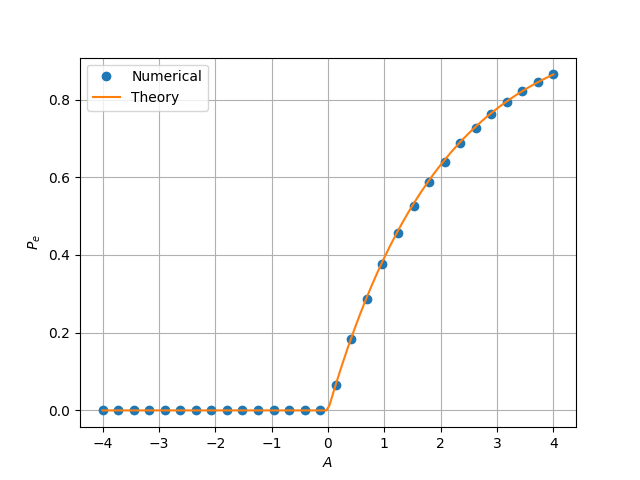
\includegraphics[width=\columnwidth]{./figures/CDF_chi.png}
    \caption{The CDF of $V$}
    \label{fig:chi_cdf}
    \end{figure}

    \begin{figure}
        \centering
        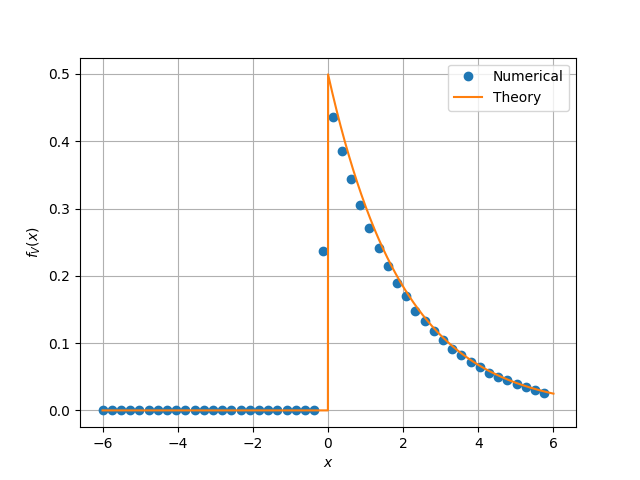
\includegraphics[width=\columnwidth]{./figures/PDF_chi.png}
        \caption{The PDF of $V$}
        \label{fig:chi_pdf}
        \end{figure}

The graphs are plotted in Fig. \ref{fig:chi_cdf}

\label{eq:qn_Fv}
\item
If
%
\begin{equation}
F_{V}(x) = 
\begin{cases}
1 - e^{-\alpha x} & x \geq 0 \\
0 & x < 0,
\end{cases}
\end{equation}
%
find $\alpha$.
%
\\
\solution We will assume that $X_1$ and $X_2$ are i.i.d. 
Let
\begin{align}
    X_1 = r \cos{\theta} \\
    X_2 = r \sin{\theta} \\
\end{align}
 The Jacobian Matrix is then defined as: 
 \begin{align}
    J     & = \myvec{\frac{\delta x_1}{\delta r}    & \frac{\delta x_1}{\delta \theta} \\ \frac{\delta x_2}{\delta r} & \frac{\delta x_2}{\delta \theta}}\\
    J &=  \myvec{\frac{\delta r \cos{\theta}}{\delta r} & \frac{\delta  r \cos{\theta}}{\delta \theta} \\ \frac{\delta r \sin{\theta}}{\delta r}  & \frac{\delta r \sin{\theta}}{\delta \theta}}\\
    J    & = \myvec{\cos\theta    & -R\sin\theta    \\ \sin\theta & R\cos\theta} \\
   \implies |J|          & = R
 \end{align}


Then, 
\begin{align}
    f_{X_1,X_2}(x_1,x_2) &= f_{X_1}(x_1)f_{X_2}(x_2) \\
    &= \frac{1}{2\pi} e^{\frac{-(x_1^2+x_2^2)}{2}} \\
    &= \frac{1}{2\pi} e^{\frac{-r^2}{2}}
\end{align}

Now, since 
\begin{align}
    f_{r, \theta}(r, \theta) &= |J|f_{X_1, X_2}(x_1, x_2)      \\   
\intertext{we have:}     
f_{R, \theta}(r, \theta) & = \frac{r}{2\pi} e^{-\frac{r^2}{2}}                                                    
\end{align}

Therefore, 
\begin{align}
    f_R(r)                   & = \int_0^{2\pi} f_{R, \theta}(r, \theta)                                                     \\
    & = \int_0^{2\pi} \frac{r}{2\pi} e^{-\frac{r^2}{2}} d\theta                                    \\
    & = r e^{-\frac{r^2}{2}}                                                                       \\
\end{align}

We then have:
\begin{align}
    F_R(r) &= \pr{R \leq r} \\
    &= \int _{0} ^r f_R(r) dr
    &= 1 - e^{-\frac{r^2}{2}}
\end{align}

$F_V(x)$ is given by:

\begin{align}
    F_V(x) &= F_{X_1^2+X_2^2}(x) \\
    &= F_{R^2}{x} \\
    &= \pr{R^2 \leq x} \\
    &= \pr{R \leq \sqrt{x}} 
\end{align}

Therefore, 


\begin{align}
    F_V(x) = 
    \begin{cases}
        0, & x \in x < 0 \\
        1 - e^{-\frac{x}{2}}, & x \geq  0\\
    \end{cases}
\end{align}

Comparing with Eq. \ref{eq:qn_Fv} we get:

\begin{align}
    \alpha = \frac{1}{2}
\end{align}


\item
\label{ch3_raleigh_sim}
Plot the CDF and PDF of
%
\begin{equation}
A = \sqrt{V}
\end{equation}
%
\\
\solution
Use the function "ray" in \textbf{exrand.c} and execute:
\begin{lstlisting}
    gcc exrand.c
    ./a.out
\end{lstlisting}

Add the functions "ray\_pdf" and "ray\_cdf" to \textbf{functions.py} and execute 
the below files:
\begin{lstlisting}
    python3 pdf_plot.py
    python3 cdf_plot.py
\end{lstlisting}

The graphs are plotted in Fig. \ref{fig:ray_cdf}


\begin{figure}
    \centering
    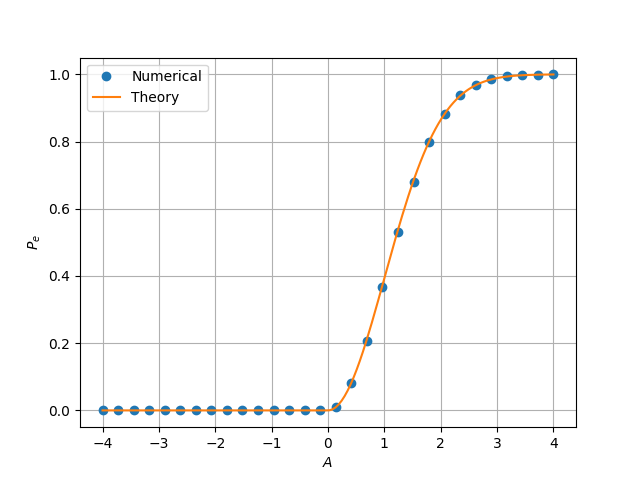
\includegraphics[width=\columnwidth]{./figures/CDF_ray.png}
    \caption{The CDF of $A$}
    \label{fig:ray_cdf}
    \end{figure}

    \begin{figure}
        \centering
        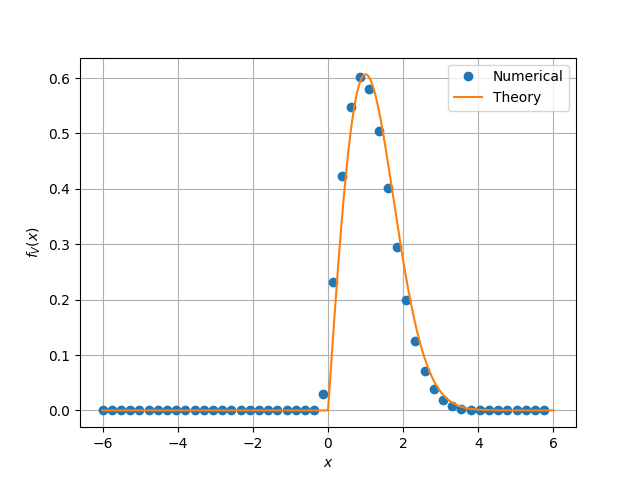
\includegraphics[width=\columnwidth]{./figures/PDF_ray.png}
        \caption{The PDF of $A$}
        \label{fig:ray_pdf}
        \end{figure}


       


\end{enumerate}
















\section{Conditional Probability}
\begin{enumerate}[label=\thesection.\arabic*
,ref=\thesection.\theenumi]
\item
\label{ch4_sim}
Plot 
\begin{equation}
P_e = \pr{\hat{X} = -1|X=1}
\end{equation}
%
for 
\begin{equation}
Y = AX+N,
\end{equation}
where $A$ is Raleigh with $E\sbrak{A^2} = \gamma, N \sim \gauss{0}{1}, X \in \brak{-1,1}$ for $0 \le \gamma \le 10$ dB.
%
\item
Assuming that $N$ is a constant, find an expression for $P_e$.  Call this $P_e(N)$
%
\item
%
\label{ch4_anal}
For a function $g$,
\begin{equation}
E\sbrak{g(X)} = \int_{-\infty}^{\infty}g(x)p_{X}(x)\, dx
\end{equation}
%
Find $P_e = E\sbrak{P_e(N)}$.
%
\item
Plot $P_e$ in problems \ref{ch4_sim} and \ref{ch4_anal} on the same graph w.r.t $\gamma$.  Comment.
		\end{enumerate}
\section{Two Dimensions}
Let 
\begin{equation}
\mbf{y} = A\mbf{x} + \mbf{n},
\end{equation}
where 
\begin{align}
x &\in \brak{\mbf{s}_0,\mbf{s}_1}, 
\mbf{s}_0 = 
\begin{pmatrix}
1 
\\
0
\end{pmatrix},
\mbf{s}_1 = 
\begin{pmatrix}
0 
\\
1
\end{pmatrix}
\\
\mbf{n} &= 
\begin{pmatrix}
n_1
\\
n_2
\end{pmatrix},
n_1,n_2 \sim \gauss{0}{1}.
\end{align}
%
\begin{enumerate}[label=\thesection.\arabic*
,ref=\thesection.\theenumi]
%%
\item
\label{ch5_fsk}
Plot 
%
\begin{equation}
\mbf{y}|\mbf{s}_0 \text{ and } \mbf{y}|\mbf{s}_1
\end{equation}
%
on the same graph using a scatter plot.
%
\item
For the above problem, find a decision rule for detecting the symbols $\mbf{s}_0 $ and $\mbf{s}_1$.
%
\item
Plot 
\begin{equation} 
P_e = \pr{\hat{\mbf{x}} = \mbf{s}_1|\mbf{x} = \mbf{s}_0}
\end{equation}
with respect to the SNR from 0 to 10 dB.
%
\item
Obtain an expression for $P_e$. Verify this by comparing the theory and simulation plots on the same graph.
%
		\end{enumerate}








\end{document}
